\documentclass[border=2pt]{standalone}
\usepackage{tikz}
\usepackage{pgfplots}
\pgfplotsset{compat=1.18}
\definecolor{mprimary}{HTML}{2C3E6B}
\definecolor{maccent}{HTML}{C8A951}
\definecolor{mgood}{HTML}{5B8C6B}
\definecolor{mbad}{HTML}{B85450}
\definecolor{mgray}{HTML}{9E9E9E}
\begin{document}
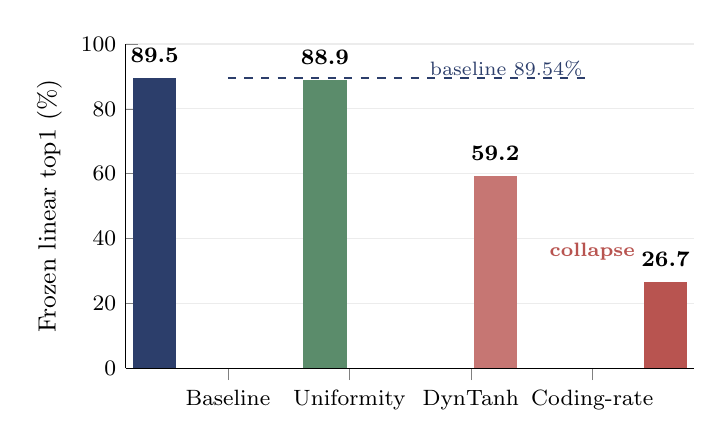
\begin{tikzpicture}
\begin{axis}[
    width=8.8cm, height=5.7cm,
    ybar, bar width=0.55cm,
    ylabel={Frozen linear top1 (\%)},
    ymin=0, ymax=100,
    ymajorgrids=true,
    grid style={mgray!20},
    axis x line*=bottom,
    axis y line*=left,
    symbolic x coords={Baseline,Uniformity,DynTanh,{Coding-rate}},
    xtick={Baseline,Uniformity,DynTanh,{Coding-rate}},
    xticklabel style={font=\footnotesize, align=center},
    tick label style={font=\footnotesize},
    label style={font=\small},
    nodes near coords,
    point meta=explicit symbolic,
    nodes near coords style={font=\footnotesize\bfseries, yshift=2pt},
    enlarge x limits=0.28]
  \addplot[draw=none, fill=mprimary] coordinates {(Baseline,89.54) [89.5]};
  \addplot[draw=none, fill=mgood] coordinates {(Uniformity,88.88) [88.9]};
  \addplot[draw=none, fill=mbad!80] coordinates {(DynTanh,59.24) [59.2]};
  \addplot[draw=none, fill=mbad] coordinates {({Coding-rate},26.73) [26.7]};
  \draw[mprimary, thick, dashed] (axis cs:Baseline,89.54) -- (axis cs:{Coding-rate},89.54);
  \node[font=\scriptsize, mprimary, anchor=east] at (axis cs:{Coding-rate},92.5) {baseline 89.54\%};
  \node[font=\scriptsize\bfseries, mbad, align=center] at (axis cs:{Coding-rate},36) {collapse};
\end{axis}
\end{tikzpicture}
\end{document}
